\section{Electromagnetismo}

\subsection{Introducción}

El imán es un cuerpo o dispositivo con un magnetismo significativo, de forma que atrae a otros imanes o metales ferromagnéticos (por ejemplo, hierro, cobalto, níquel y aleaciones de estos). El magnetismo es el conjunto de fenómenos físicos mediados por campos magnéticos, que son una representación matemática del modo en que las fuerzas magnéticas interactúan y se distribuyen en el espacio.

\begin{figure}[ht]
  \centering
  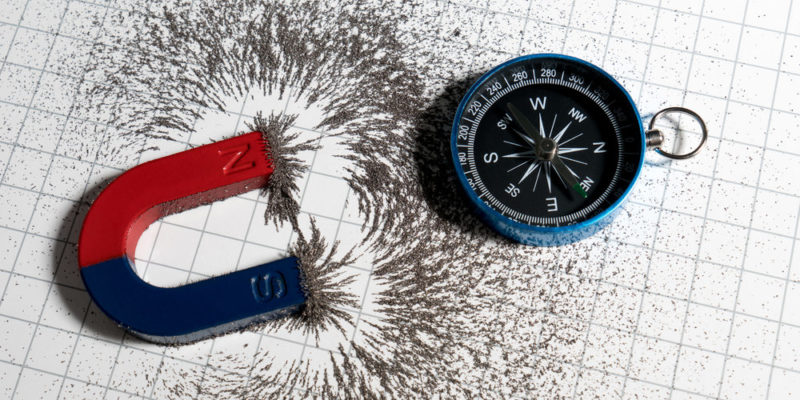
\includegraphics[width=0.5\textwidth]{iman-brujula.jpg}
  \caption{Limaduras de hierro y brújula afectados por un imán de herradura}
  \label{fig:iman}
\end{figure}

Como se puede apreciar en la figura \ref{fig:iman}, todos los imanes poseen dos polos, llamados \textit{polo norte} y \textit{polo sur}. Cualquiera de los polos de un imán atrae a un objeto ferromagnético no magnetizado, pero, al igual que pasaba con las cargas eléctricas, los polos iguales se repelen y los polos opuestos se atraen. Es decir polo norte y polo sur se atraen, mientras que polo norte y polo norte (o sur y sur) se repelen.

La relación entre la electricidad y el magnetismo fue descubierta en 1819, cuando en el transcurso de una demostración en una conferencia, el científico danés Hans Christian Oersted descubrió que una corriente eléctrica en un alambre desviaba la aguja de una brújula cercana. Durante 1820, Faraday y Joseph Henry demostraron, de manera independiente relaciones adicionales entre la electricidad y el magnetismo. Mostraron que es posible crear una corriente eléctrica en un circuito ya sea moviendo un imán cerca de él o variando la corriente de algún circuito cercano. Estas observaciones demuestran que una variación en un campo magnético crea un campo eléctrico. Años después, el trabajo teórico de Maxwell demostró que lo contrario también es cierto: un campo eléctrico que varía crea un campo magnético.

\subsection{Magnetismo}

Tal vez el concepto de polos magnéticos parezca similar al de carga eléctrica, y los polos norte y sur parezcan análogos a las cargas positiva y negativa. No obstante, tal analogía puede ser errónea. Si bien las cargas positiva y negativa existen aisladas, no hay evidencia experimental de que exista un polo magnético aislado.

Los imanes siempre se encuentran como dipolos magnéticos (norte y sur), y no se ha comprobado la existencia los monopolos magnéticos.

\subsubsection{Campo Magnético}

Al igual que el campo eléctrico, el magnético es un \hl{\textit{campo vectorial}}, es decir, una cantidad vectorial asociada con cada punto del espacio. La existencia de un campo magnético en algún punto del espacio puede determinarse midiendo la magnitud de la \textbf{fuerza magnética} que ejerce el campo sobre una partícula de prueba ubicada en ese punto.

El magnetismo es un fenómeno físico asociado al movimiento de cargas eléctricas, que da lugar a fuerzas de atracción o repulsión entre materiales. Se manifiesta principalmente a través de los campos magnéticos, los cuales son representaciones vectoriales que describen la influencia que una corriente eléctrica o un material magnético ejerce en su entorno.

Desde un punto de vista fundamental, \hl{el origen del magnetismo reside en el movimiento de cargas eléctricas} a nivel microscópico, particularmente en el espín y el momento orbital de los electrones en los átomos. En materiales como el hierro, cobalto y níquel, estos momentos magnéticos atómicos se alinean de manera colectiva, generando imanes permanentes.

El campo magnético se representa mediante el vector \(\vec{B}\), cuya unidad en el Sistema Internacional es el tesla (T)\footnote{Un tesla equivale a: \(T=\frac{N}{C\, m/s}\)}. La interacción de una carga en \textbf{movimiento} \(q\) con un campo magnético está regida por la fuerza magnética, expresada como:
\begin{equation}
  \vec{F}_B = q\vec{v} \times \vec{B}
  \label{eq:fuerza_magnética}
\end{equation}
donde \(\vec{v}\) es el vector velocidad de la partícula. Esta fuerza es perpendicular tanto a la dirección de la velocidad como a la del campo magnético.

\begin{figure}[ht]
  \centering
  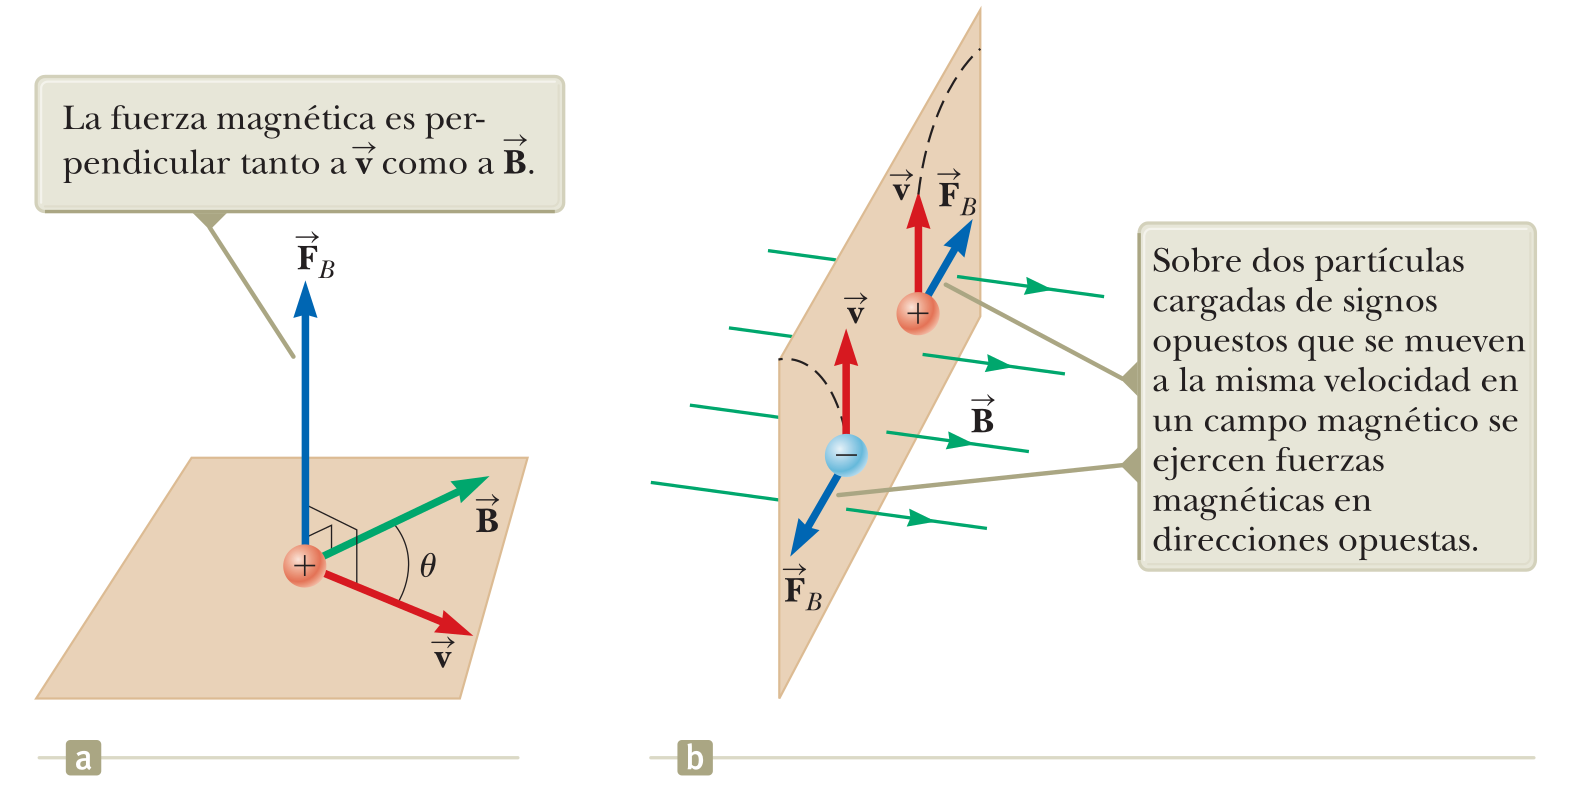
\includegraphics[width=0.8\textwidth]{magnetic_force.png}
  \caption{Partículas con carga atravesando un campo magnético \(\vec{B}\) con una velocidad \(\vec{v}\)}
\end{figure}

Si se conoce el ángulo \(\theta\) entre el vector velocidad \(\vec{v}\) y el campo magnético \(\vec{B}\) la fuerza se puede calcular como:
\[
  \vec{F}_B = \abs{q} v B \sin(\theta) \hat{r}
\]
donde \(\hat{r}\) es un vector normal al plano formado por los vectores \(\vec{v}\) y \(\vec{B}\). 

Comparando la fuerza magnética con la fuerza eléctrica se puede ver que el vector \(\vec{F}_B\) es perpendicular al campo magnético y a la velocidad y desplazamiento de la partícula, mientras que \(\vec{F}_e\) se ejerce sobre la dirección del campo eléctrico. En base a esto, vemos que \(\vec{F}_B\) no realiza trabajo ni cambia la energía del sistema carga-campo. 

\begin{tcolorbox}[myconclusion]
  Con base en este último enunciado y también con el teorema trabajo-energía cinética, se concluye que la energía cinética de una partícula cargada que se mueve a través de un campo magnético \textbf{no} puede ser modificada sólo por el campo magnético. El campo magnético puede modificar la dirección del vector velocidad, pero no puede cambiar la rapidez ni la energía cinética de la partícula.
\end{tcolorbox}

\subparagraph{Pregunta:}

\noindent ¿Qué tipo de fuerza es siempre perpendicular a la trayectoria de una partícula?

\vspace{3pt}

\noindent La \textbf{fuerza centrípeta}. Entonces, la fuerza magnética es una fuerza centrípeta para una partícula cargada y en movimiento. Por lo tanto podemos ocupar todas las ecuaciones del movimiento circular.

\begin{figure}[ht]
  \centering
  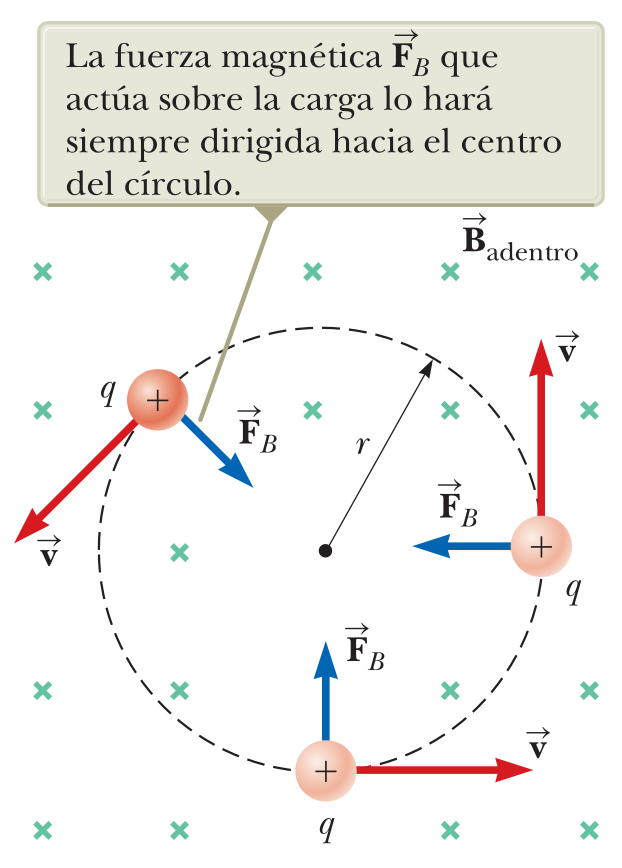
\includegraphics[width=0.35\textwidth]{centipet_force.png}
  \caption{Fuerza magnética para una partícula con velocidad \(v\) y un campo magnético entrante.}
  \label{fig:centripet_force}
\end{figure}

\paragraph{Recordatorio de movimiento circular}

\subparagraph{Posición angular (\(\theta\))}

La posición angular indica el ángulo barrido respecto a un eje fijo.
\[
\theta(t) = \theta_0 + \omega_0 t + \frac{1}{2} \alpha t^2
\]
donde:
\begin{itemize}
  \item \(\theta_0\) es la posición angular inicial,
  \item \(\omega_0\) es la velocidad angular inicial,
  \item \(\alpha\) es la aceleración angular.
\end{itemize}

\subparagraph{Velocidad angular (\(\omega\))}

La velocidad angular mide el cambio de la posición angular respecto al tiempo.
\[
\omega(t) = \omega_0 + \alpha t
\]
Y también:
\[
\omega^2 = \omega_0^2 + 2\alpha(\theta - \theta_0)
\]
Esta última es útil si desea eliminar el tiempo de la ecuación. Si se pide relacionar el tipo de movimiento con la frecuencia:
\[
  \omega = 2 \pi f
\]

\subparagraph{Aceleración angular (\(\alpha\))}  

Es la razón de cambio de la velocidad angular:
\[
\alpha = \frac{d\omega}{dt}
\]

En general en los problemas de magnetismo que aborda la materia la aceleración angular será cero.

\subparagraph{Velocidad tangencial (\(v_t\))}  

La velocidad lineal de un punto situado a una distancia \( r \) del eje de rotación es:
\[
v_t = r \, \omega
\]
La dirección de \( v_t \) es siempre tangente a la trayectoria circular.

\subparagraph{Aceleración centrípeta (\(a_c\))}

La aceleración centrípeta está directamente relacionada con la velocidad tangencial en el movimiento circular. Su relación es:
\[
a_c = \frac{v_t^2}{r}
\]
Esta aceleración siempre está presente y se encarga de cambiar la dirección del vector velocidad en cada punto.

\subparagraph{Aceleración tangencial (\(a_t\))}  

La aceleración tangencial está asociada al cambio en el módulo de la velocidad tangencial y por lo tanto, a la aceleración angular:
\[
a_t = r \, \alpha
\]

\subparagraph{Fuerza centrípeta (\(F_c\))}

La fuerza necesaria para mantener un cuerpo en movimiento circular uniforme (o no uniforme) está dirigida hacia el centro de la trayectoria:
\[
F_c = m \frac{v_t^2}{r} = m r \omega^2
\]
donde \( m \) es la masa del objeto.

\subsection{Fuerza de Lorentz}

Una carga móvil con una velocidad \(\vec{v}\), en presencia tanto de un campo eléctrico \(\vec{E}\) como de un campo magnético \(\vec{B}\) es descrito por dos modelos de partícula en un campo. Experimenta a la vez una fuerza eléctrica \(q\vec{E}\) y una fuerza magnética \(q\vec{v} \times \vec{B}\). La fuerza total es la fuerza de Lorentz:

\[
  \vec{F}_B = q\vec{E} + q\vec{v} \times \vec{B}
\]

\begin{wrapfigure}{r}{0.3\textwidth}
  \centering
  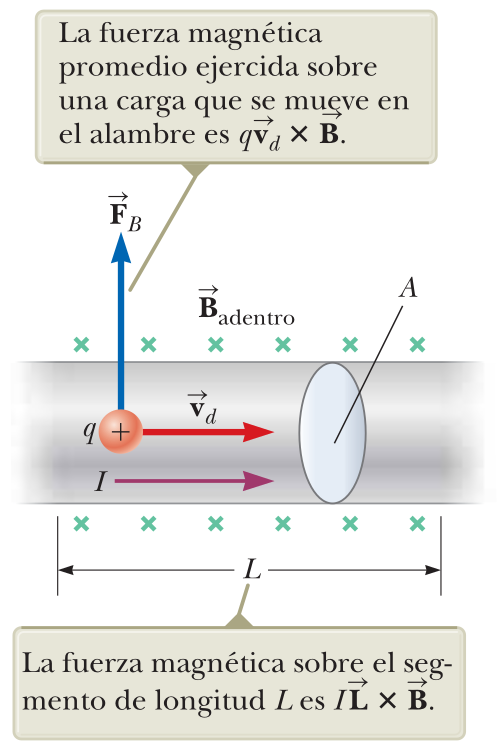
\includegraphics[width=0.3\textwidth]{lorentz.png}
  \caption{Un segmento de un alambre conduciendo corriente en un campo magnético \(\vec{B}\)}
  \label{fig:lorentz}
\end{wrapfigure}
Ahora hagamos un análisis de las fuerzas que interactúan para un cable conductor como el que se muestra en la figura \ref{fig:lorentz}. Vemos que en la figura el campo magnético es entrante. Si no circula corriente eléctrica, entonces no hay movimiento de cargas, por ende las cargas tendrán una \(v_d=0\) y la fuerza magnética será cero. Si hacemos circular cargas sobre el conductor aplicando una diferencia de potencial entre las puntas del conductor, entonces \(v_d \neq 0\) y por lo tanto existirá una fuerza magnética. 
Conviene cuantificar esta explicación considerando la longitud \(L\) del segmento y el área de sección transversal \(A\). Al tener en cuenta las dimensiones del cable, podemos expresar analizar la \textbf{fuerza total} que sentirá el cable. Sabiendo que la corriente que circula por el cable es \(I = nq v_d A\) y el volumen del cable es \(AL\) entonces: 
\[
  \vec{F}_B = (q\vec{v}_d \times \vec{B})nAL
\]
Reemplazando \(I=qn \vec{v}_d A\) en la expresión:
\[
  \vec{F}_B = I\vec{L} \times \vec{B}
\]
donde \(\vec{L}\) es un vector que apunta en la dirección de la corriente \(I\) y tiene una magnitud igual a la longitud \(L\). Si se expresa el producto vectorial como el módulo de los vectores por el seno del ángulo entre ellos:
\begin{equation}
  \boxed{F_B = IL \cdot B \, \sin(\theta)}
\end{equation}

\subsection{Flujo Magnético}

Definimos el \textbf{flujo magnético} \(\Phi_B\) a través de una superficie igual que definimos el flujo eléctrico en relación con la ley de Gauss en la sección \ref{sec:flujo_electrico}. 

El flujo magnético es una magnitud escalar que cuantifica la cantidad de campo magnético que atraviesa una superficie dada. Matemáticamente, se define como la integral del producto escalar entre el campo magnético \(\vec{B}\) y el vector diferencial de área \(d\vec{A}\) de la superficie:

\[
\Phi_B = \int_S \vec{B} \cdot d\vec{A}
\]
donde:
\begin{itemize}
  \item \(\Phi_B\) es el flujo magnético,
  \item \(S\) es la superficie sobre la que se calcula el flujo,
  \item \(\vec{B}\) es el vector del campo magnético,
  \item \(d\vec{A}\) es un elemento diferencial de área, cuyo módulo es el área diferencial y cuya dirección es perpendicular a la superficie, siguiendo la convención del sentido positivo (normal saliente en una superficie cerrada).
\end{itemize}

Al igual que el flujo eléctrico, el flujo magnético mide cuántas ``líneas de campo magnético'' atraviesan una superficie. Si el campo es perpendicular a la superficie, el flujo es máximo; si es paralelo, el flujo es nulo.

En el caso especial donde el campo magnético es uniforme y la superficie es plana, la expresión se simplifica a:
\[
\Phi_B = B A \cos\theta
\]
donde:
\begin{itemize}
  \item \(B\) es la magnitud del campo magnético,
  \item \(A\) es el área de la superficie,
  \item \(\theta\) es el ángulo entre el vector \(\vec{B}\) y el vector normal a la superficie.
\end{itemize}

La unidad de flujo magnético en el Sistema Internacional es el weber (Wb), donde: \(1 \, \text{Wb} = 1 \, \text{T} \cdot \text{m}^2\)

\subsection{Momento de torsión sobre una espira de corriente}

\subsubsection{Introducción general}

Cuando una espira de corriente se coloca en un campo magnético uniforme, cada segmento de la espira experimenta una fuerza magnética dada por la ley de Lorentz. Estas fuerzas no se cancelan completamente en su efecto mecánico: aunque su suma vectorial puede ser nula (es decir, no producen una traslación neta de la espira), sí generan un momento de torsión o torque que tiende a rotarla.

Esta rotación es esencial para entender el funcionamiento de dispositivos como los motores eléctricos, galvanómetros y otros sistemas electromecánicos.

Primero, teniendo en cuenta que un pequeño elemento de espira experimenta un diferencial de \(\vec{F}_B\). La fuerza magnética diferencial sobre un elemento de corriente es:
\[
  d\vec{F} = I \, d\vec{l} \times \vec{B}
\]
donde:
\begin{itemize}
  \item \(I\) es la corriente (supuesta constante),
  \item \(d\vec{l}\) es el vector diferencial de longitud en la dirección de la corriente,
  \item \(\vec{B}\) es el campo magnético.
\end{itemize}
\begin{tcolorbox}[myconclusion]
  Esta fuerza es perpendicular tanto al elemento de corriente como al campo magnético.
\end{tcolorbox}

\subsubsection{Definición de momento de torsión}

El momento de torsión o torque \(\vec{\tau}\) respecto a un punto (usualmente el centro de masas o el centro geométrico de la espira) es:
\[
\vec{\tau} = \oint \vec{r} \times d\vec{F} =\int_S \vec{r} \times d\vec{F}
\]
donde:
\begin{itemize}
  \item \(\vec{r}\) es el vector de posición del elemento de corriente respecto al punto de referencia,
  \item \(d\vec{F}\) es la fuerza diferencial que actúa sobre dicho elemento.
  \item \(S\) es la curva que representa la espira de corriente.
\end{itemize}

Para realizar el cálculo del momento de torsión sobre una espira plana, supongamos que tenemos una espira plana de forma arbitraria, con una corriente \(I\), en presencia de un campo magnético uniforme \(\vec{B}\).

Utilizando las expresiones anteriores y sustituyendo \(d\vec{F}\), obtenemos:

\[
\vec{\tau} = \int_S \vec{r} \times (I \, d\vec{l} \times \vec{B})
\]

Aplicando la propiedad del producto vectorial triple:
\[
\vec{a} \times (\vec{b} \times \vec{c}) = (\vec{a} \cdot \vec{c})\vec{b} - (\vec{a} \cdot \vec{b})\vec{c}
\]
obtenemos:
\[
\vec{\tau} = I \int_S \left[ (\vec{r} \cdot \vec{B}) d\vec{l} - (\vec{r} \cdot d\vec{l}) \vec{B} \right]
\]

Ahora, si analizamos los términos:
\begin{enumerate}
  \item El primer término, \( (\vec{r} \cdot \vec{B}) d\vec{l} \), es complicado de integrar directamente, pero bajo simetrías adecuadas, puede tratarse convenientemente.
  \item El segundo término, \((\vec{r} \cdot d\vec{l})\), es el doble del área orientada de la espira (relacionado con el teorema de Stokes).
\end{enumerate}

En resumen, después de un tratamiento matemático (que puedo desarrollar si usted lo desea), se demuestra que:
\[
\vec{\tau} = \vec{\mu} \times \vec{B}
\]
donde \(\vec{\mu}\) es el momento dipolar magnético de la espira, definido como:
\[
\vec{\mu} = I \, \vec{A}
\]
Aquí:
\begin{itemize}
  \item \(I\) es la corriente,
  \item \(\vec{A}\) es el vector área de la espira: su magnitud es el área \(A\) de la espira, y su dirección es normal al plano de la espira, siguiendo la regla de la mano derecha respecto al sentido de la corriente.
\end{itemize}

\begin{tcolorbox}[myconclusion]
  La fuerza neta sobre una espira de corriente un un campo magnético uniforme es igual a cero. Sin embargo, el par de torsión neto en general no es igual a cero.
\end{tcolorbox}

Si el momento magnético \(\vec{\mu}\) es paralelo o antiparalelo al campo \(\vec{B}\), no hay momento de torsión (\(\tau = 0\)). Si \(\vec{\mu}\) es perpendicular a \(\vec{B}\), el momento de torsión es máximo. El torque tiende a alinear \(\vec{\mu}\) con \(\vec{B}\), en analogía con el comportamiento de un dipolo eléctrico en un campo eléctrico.

\paragraph{Expresión escalar del torque}

La magnitud del momento de torsión es:

\begin{equation}
  \boxed{\tau = \mu B\sin\theta}
\end{equation}
donde \(\theta\) es el ángulo entre \(\vec{\mu}\) y \(\vec{B}\).
\begin{tcolorbox}[myconclusion]
  La dirección del torque se obtiene por la regla de la mano derecha aplicada al producto vectorial \(\vec{\mu} \times \vec{B}\).
\end{tcolorbox}
\begin{figure}[ht]
  \centering
  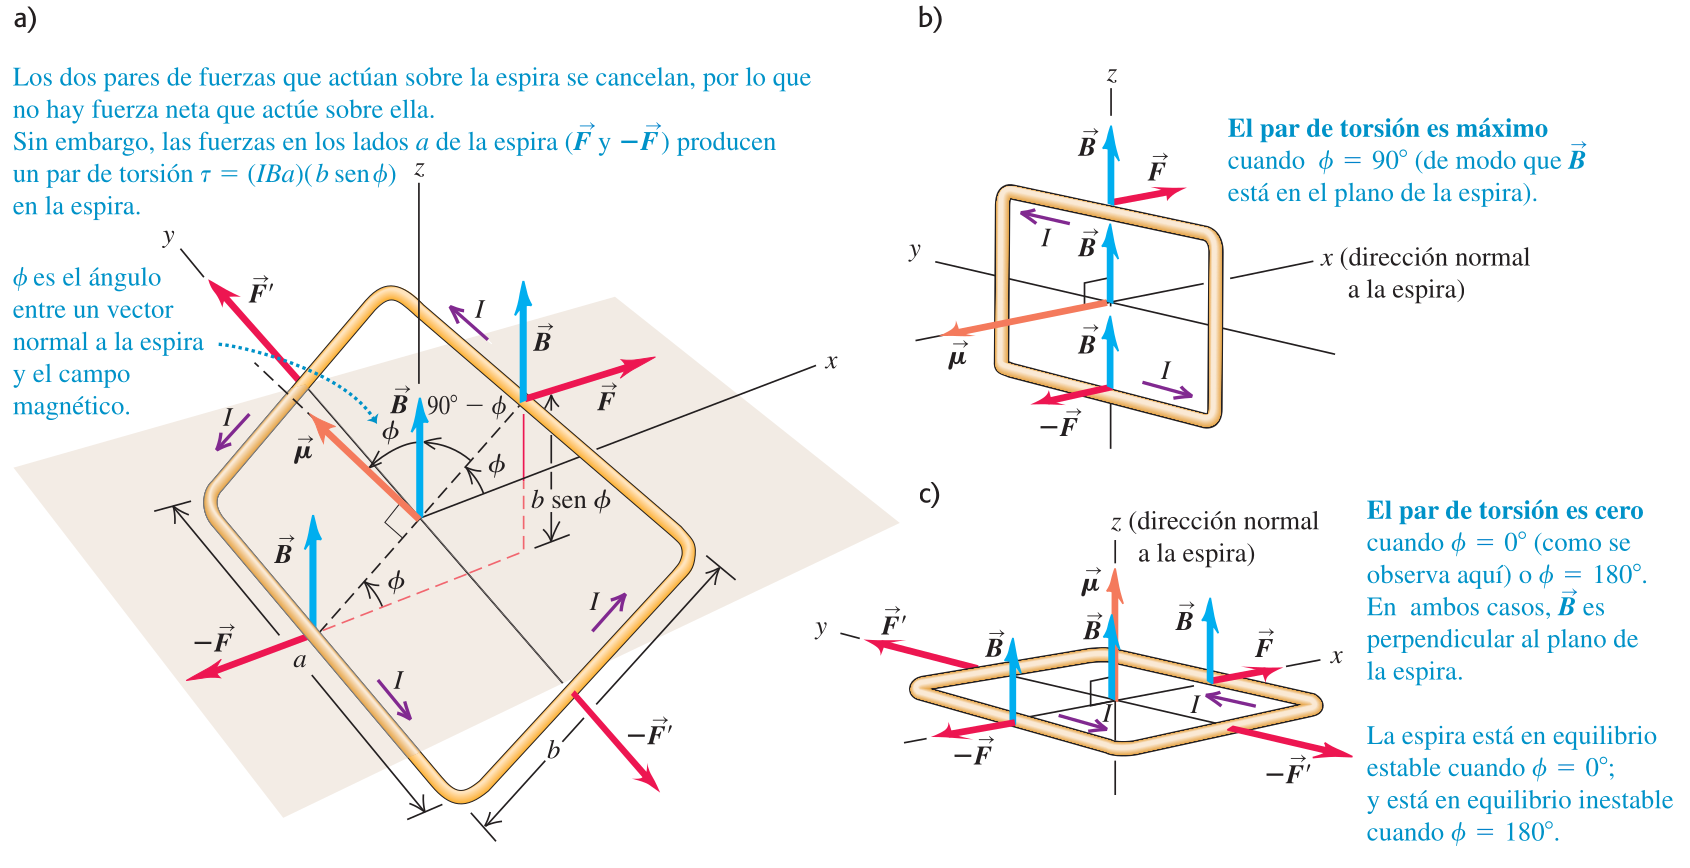
\includegraphics[width=1\textwidth]{par.png}
  \caption{Cálculo del par de torsión sobre una espira que conduce corriente en un campo magnético uniforme.}
\end{figure}